\chapter{Splotowe sieci neuronowe}
Splotowe sieci neuronowe są wielowarstwowymi sieciami jednokierunkowymi. Charakteryzuje je~możliwość
wykrywania wzorców występujących w~różnych fragmentach przetwarzanego obrazu (np. rozpoznawanie oka
w~dowolnym fragmencie obrazka). Zasada ich~działania była inspirowana neurobiologią, a~mianowicie analizowano
sposób przetwarzania informacji przez~ośrodek wzrokowy kota.

\section{Filtry splotowe}
Splot dyskrentny jako pojęcie matematyczne jest zdefiniowany w~następujący sposób:
$$ f\ast g[n]\defeq \sum\limits_{m=-\infty}^{\infty}f[m]g[n-m] = \sum\limits_{m=-\infty}^{\infty}f[n-m]g[m]$$

W~cyfrowym przetwarzaniu obrazów filtry splotowe znajdują bardzo szerokie zastosowanie, gdyż w~zależności
od~dobranej maski filtra, osiągane są różne rezultaty. Przykładowe filtry splotowe:
\begin{itemize}
  \item filtr Gaussa (wygładzanie),
  \item filtr Laplace'a (wyostrzanie).
\end{itemize}
Maski dla~wymienionych filtrów są~z~góry ustalone i~nie~ulegają zmianie w~czasie działania algorytmu. Splotowa
sieć neuronowa zamiast wykorzystywać z~góry określone maski, ,,uczy się ich'', a~więc stara się~tak dobrać
ich~wartości, aby~jak~najlepiej rozpoznawać wyznaczone obiekty na~obrazach. Poszczególnym wartościom
w~masce filtra odpowiadają wagi splotowej sieci neuronowej. 

\subsection{Padding}
Przy~stosowaniu filtrów splotowych pojawia się problem: jaką wartość powinny otrzymać piksele obrazka
znajdujące się na jego krawędzi. Jest on~rozwiązywany poprzez rozszerzanie obrazka o~dodatkowe piksele
na~jego krawędziach. Można tego dokonać m.in. poprzez:
\begin{itemize}
  \item rozszerzenie obrazka o~czarne piksele (tzw.~\textit{zero-padding}),
  \item rozszerzenie obrazka odbicia lustrzane pikseli przy krawędziach.
\end{itemize}

\section{Inferencja}
W~trakcie działania sieci na~obrazie dokonywanie jest filtrowanie splotowe (przy wykorzystaniu różnych
filtrów). Po~takim filtrowaniu otrzymywane jest $n\cdot m$ obrazów, nazywanych mapami cech
(\textit{ang.~features maps}), gdzie n~-~liczba początkowych obrazów (tzw.~kanałów wejściowych), m~-~liczba
użytych filtrów.

Po~dokonaniu filtrowania splotowego obrazy są skalowane na~mniejsze (tzw.~faza pooling/subsampling) i~znów
stosowane są~filtry splotowe. Oba kroki (filtrowanie i~skalowanie) są~powtarzane wielokrotnie
(zależy od~liczby warstw sieci), aż~do~osiągnięcia odpowiednio wyskokopoziomowych cech. Liczba warstw oraz
liczba filtrów splotowych wykorzystanych w każdej z~nich jest ustalana podczas fazy projektowania sieci.

\begin{figure}[H]
	\centering
	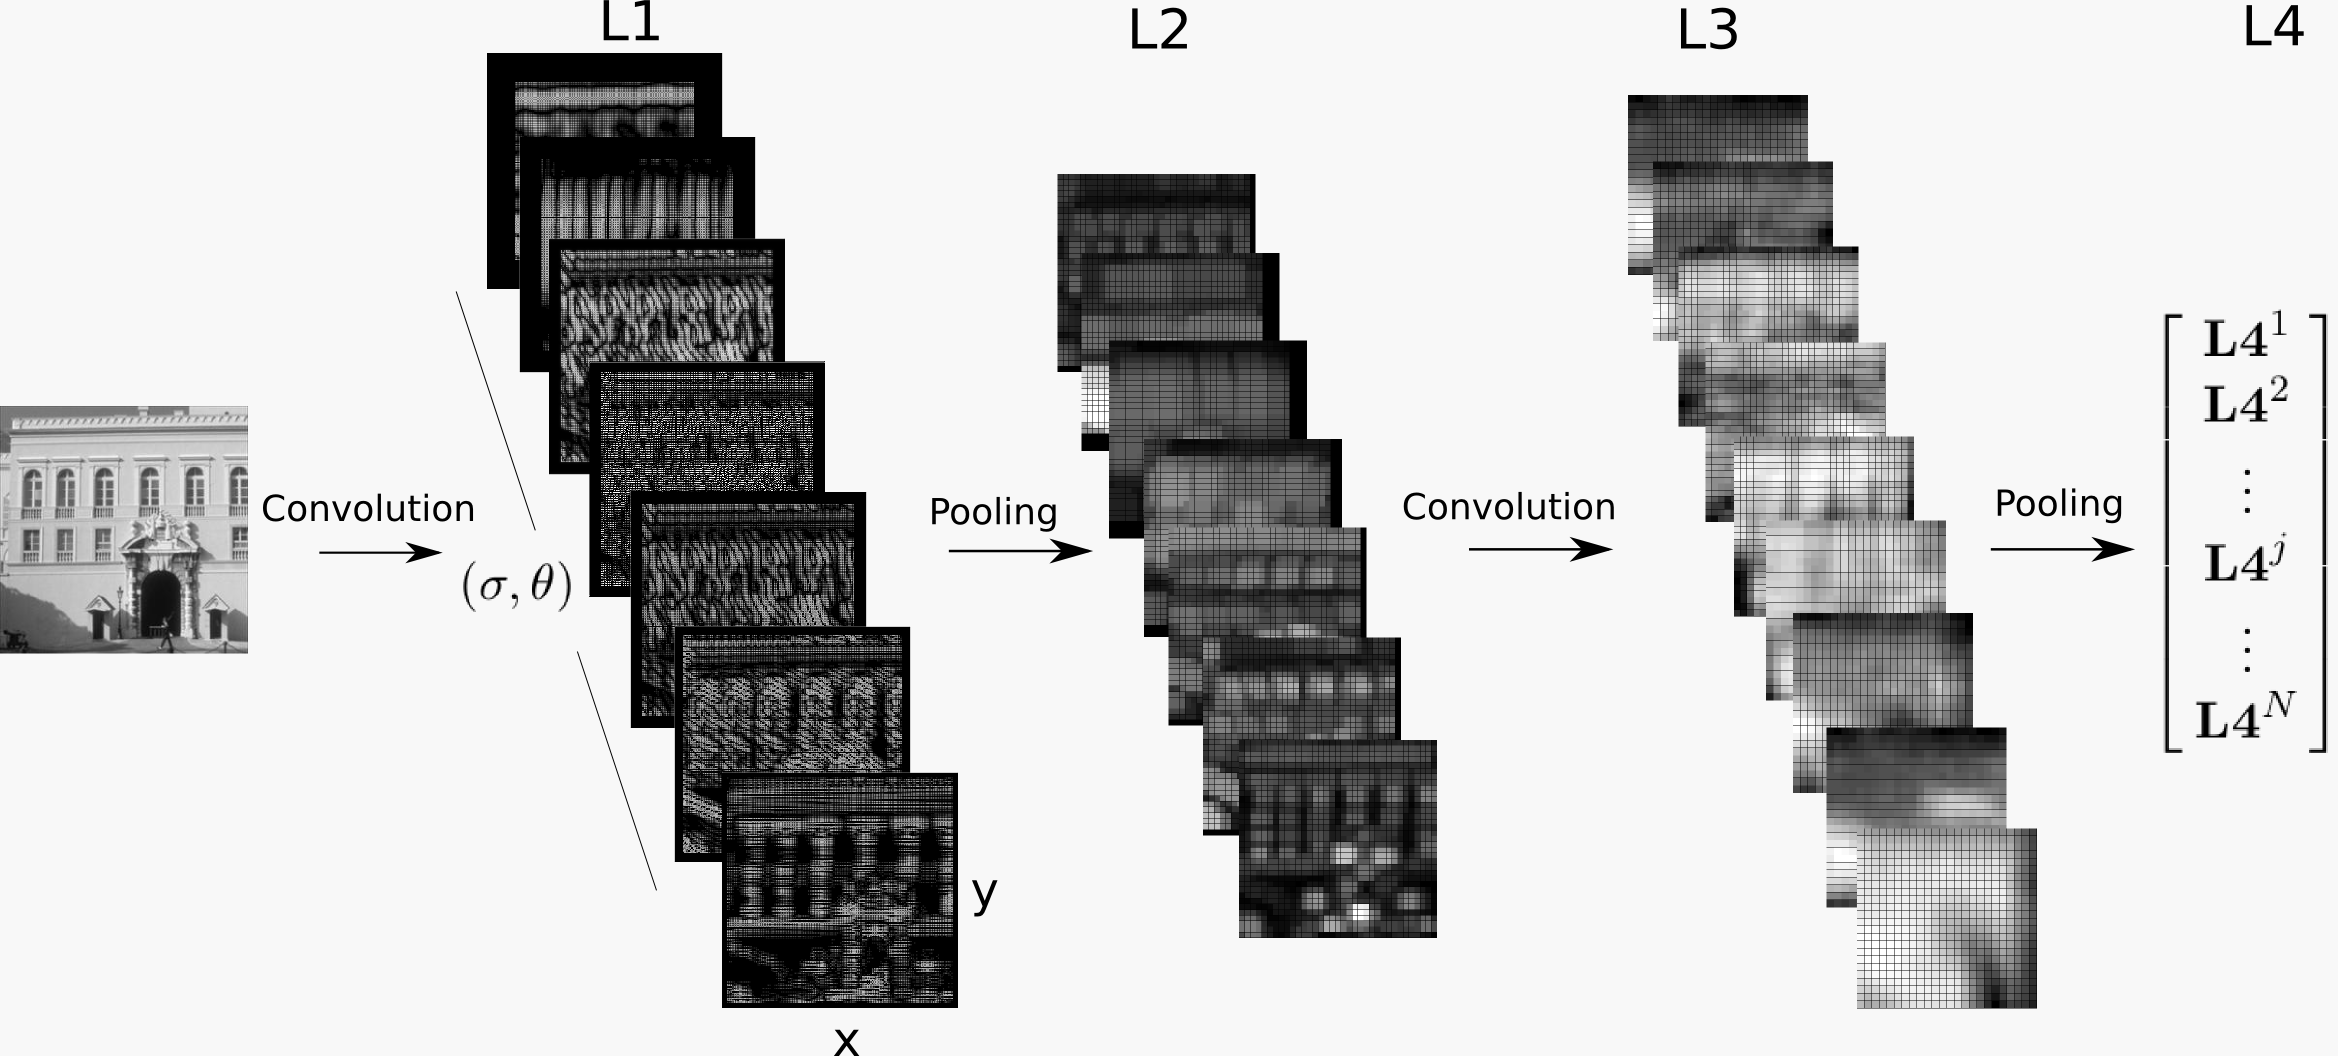
\includegraphics[width=\linewidth]{img/convnet.png}
\end{figure}

Ostatnią warstwą sieci (zazwyczaj otrzymującą dużo bardzo małych obrazów) jest warstwa zawierająca neurony
sigmoidalne. Każdy neuron warstwy wyjściowej jest połączony ze~wszystkimi wartościami otrzymanymi na~wyjściu
poprzedniej warstwy.

\subsection{Skalowanie}
Po zastosowaniu n różnych filtrów splotowych w~danej warstwie na m różnych mapach cech, powstaje $n\cdot m$
kolejnych map cech. Stąd ilość przetwarzanych danych szybko rośnie wraz z~dokładaniem kolejnych warstw
w~sieci. Aby temu przeciwdziałać stosuje się skalowanie obrazów pomiędzy warstwami dokonującymi splotu.
Najczęściej obraz skalowany jest poprzez:
\begin{enumerate}
  \item podzielenie obrazka na~nienachodzące na~siebie kwadratowe obszary,
  \item wybranie z~każdego obszaru piksela o~największej wartości (tzw.~\textit{max-pooling}). 
\end{enumerate}

Alternatywnie, w drugim kroku algorytmu można wybrać medianę wartości pikseli\\
(\textit{ang.~mean-pooling}) lub~wartość średnią (\textit{average-pooling}).

\subsection{Możliwe ulepszenia sieci}
\subsubsection{Lokalna normalizacja kontrastu}
W~sieciach splotowych często stosowanym zabiegiem, mającym na~celu zapewnienie lepszej jakości klasyfikacji jak również
szybszego uczenia, jest normalizacja danych. Operacja normalizacji może być interpretowana jako kolejna warstwa
umieszczana w~sieci na~tej~samej zasadzie, co~warstwa dokonująca splotu czy~warstwa skalująca.

\textbf{Lokalna normalizacja kontrastu}\cite{HOG} (\textit{ang.~local contrast normalization}) polega na~zapewnieniu,
że~wartości pikseli o~tych podobnych współrzędnych, jednak należące do~różnych map cech, należą do~rozkładu normalnego
o~odchyleniu standardowym równym 1 i średniej równej 0. Normalizacja polega więc na~odjęciu od~wszystkich pikseli
średniej (liczonej wzdłuż różnych map cech) i~podzieleniu ich przez~odchylenie standardowe (również liczone wzdłuż
rożnych map cech).

Choć wartości odchylenia standardowego i~średniej liczone są z~uwzględnieniem wszystkich map cech, to~nie~muszą
się ograniczać do~jednego piksela. Zamiast tego mogą dotyczyć pewnego jego sąsiedztwa. Metoda ta~odpowiada
mechanizmowi obecnemu w~ośrodkach wzrokowych ssaków, u~których również dla pewnego sąsiedztwa punktu widzianego
obrazu kontrast jest normalizowany. Przykładem tego efektu jest sytuacja, w~której obiekt w~zależności od~tego,
w~jakim otoczeniu się~znajduje, wydaje się~mieć inny kolor \ref{img:chess-illusion}.

\begin{figure}[H]
	\centering
	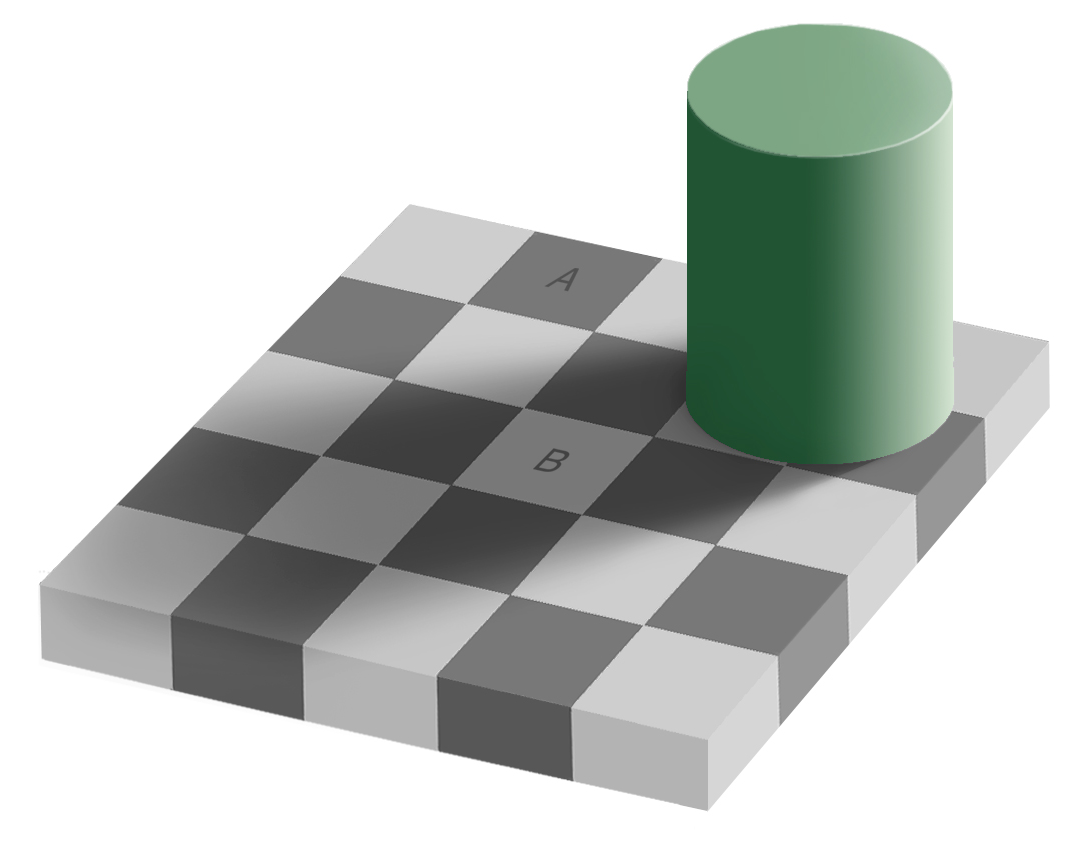
\includegraphics[width=0.8\linewidth]{img/chess-illusion.png}
	\caption{Pola A i B mają ten sam kolor}
	\label{img:chess-illusion}
\end{figure}

\subsubsection{Regularyzacja wag}
TODO
\subsubsection{Dropout}
TODO

\section{Uczenie metodą wstecznej propagacji}
Typową metodą uczenia sieci jest wsteczna propagacja błędów. W~tym celu należy obliczyć gradient funkcji
straty względem wag sieci (wartości masek filtrów splotowych) dla~warstw:
\begin{itemize}
  \item wyjściowych,
  \item skalujących,
  \item splotowych.
\end{itemize}
Obliczanie gradientu funkcji straty dla~warstw zawierających neurony sigmoidalne zostało omówione
w~sekcji (\ref{ssec:backpropagation}), stąd wyjaśnienia wymaga jedynie obliczanie gradientów dla~warstw skalujących i~splotowych.

\subsection{Obliczanie gradientu dla~warstw skalujących}
Znając gradient funkcji straty $\nabla_{y_{ijk}}l$ z~warstwy kolejnej, można w prosty sposób policzyć gradient
w~stosunku do~wejścia warstwy dla~której jest on liczony. W~przypadku, gdy~warstwa wykorzystywała algorytm
\textit{max-pooling}, gradient względem wejść warstwy przyjme wartość:
\begin{itemize}
  \item $\nabla_{x_ijk}l = \nabla_{y_{ijk}}l$, dla~pikseli, które miały maksymalną wartość w~obszarze, 
  \item $\nabla_{x_ijk}l = 0$, dla~pozostałych pikseli.
\end{itemize}

\subsection{Obliczanie gradientu dla~warstw splotowych}
Przy~wstecznej propagacji błędów z~warstwy kolejnej otrzymujemy gradient błędu względem wyjścia
aktualnej warstwy $\nabla_{y_j}l$. Do~aktualizacji wag sieci konieczne jest policzenie gradientu funkcji
straty wzlgędem wag tej warstwy.
$$ \frac{\partial E}{\partial w_{ab}} 
= \sum\limits_{i=0}^{N-m}\sum\limits_{j=0}^{N-m}\frac{\partial E}{\partial x_{ij}^l}\frac{\partial
x_{ij}^l}{\partial w_{ab}}
= \sum\limits_{i=0}^{N-m}\sum\limits_{j=0}^{N-m}\frac{\partial E}{\partial x_{ij}^l}y^{l-1}_{(i+a)(j+b)}$$
gdzie:
\begin{itemize}
  \item $N\times N$ - rozmiar mapy cech,
  \item $m\times m$ - rozmiar filtra,
  \item $x_{ij}^l$ - wartość wejścia neuronu o~wsp. (i,j) w~warstwie l,
  \item $w_{ab}$ - wartość w~masce filtra znajdująca się~na~pozycji (a,b).
\end{itemize}

Następnie należy policzyć tzw.~delty ($\frac{\partial E}{\partial x_{ij}^l}$):
$$\frac{\partial E}{\partial x_{ij}^l} = \frac{\partial E}{\partial y_{ij}^l}\frac{\partial y_{ij}^l}{\partial
x_{ij}^l} =
\frac{\partial E}{\partial y_{ij}^l}\frac{\partial}{\partial x_{ij}^l}(\sigma(x_{ij}^l))
= \frac{\partial E}{\partial y_{ij}^l}\sigma'(x_{ij}^l)
$$

Na~koniec należy policzyć gradient funkcji błędu względem wyjść warstwy poprzedniej (po~to, by~przekazać
go~do~poprzedniej warstwy):
$$ \frac{\partial E}{\partial y_{ij}^{l-1}} =
\sum\limits_{a=0}^{m-1}\sum\limits_{b=0}^{m-1} \frac{\partial E}{\partial x^l_{(i-a)(j-b)}}
\frac{\partial x^l_{(i-a)(j-b)}}{\partial y_{ij}^{l-1}} =
\sum\limits_{a=0}^{m-1}\sum\limits_{b=0}^{m-1} \frac{\partial E}{\partial x^l_{(i-a)(j-b)}}w_{ab}$$

Należy zwrócić uwagę na~dwie rzeczy: po~piersze na~to, że~podczas obliczania gradientów również wykonywany
jest splot jednak na~obrazku o~,,odwróconych'' wierszach i~kolumnach. Dodatkowo, by~móc dokonywać splotu
na~krawędziach map cech, należy zastosować \textit{zero-padding}.

\subsection{Uczenie wstępne}
W~celu lepszego zainicjowania wag sieci należy przeprowadzić uczenie wstępne. W~tym~etapie sieć zamiast uczyć
się rozpoznawania obiektów, ma~za~zadanie nauczyć się~charakteru danych wejściowych (ma~zauważać
charakterystyczne cechy, podobieństwa obiektów it.p.). Do~uczenia wstępnego wykorzystuje się~mechanizmy
uczenia nienadzorowanego, takie jak:
\begin{itemize}
  \item autoenkoder,
  \item RBM (Restricted Boltzmann Machine).
\end{itemize}

Uczenie wstępne przebiega w~następujący sposób:
\begin{enumerate}
  \item wyodrębnienie losowych fragmentów obrazka (tzw.~łatki),
  \item uczenie mechanizmu uczenia nienadzorowanego (np.~RBM),
  \item zainicjowanie wag uczonej warstwy wagami z~tego~mechanizmu,
  \item policzenie map cech dla~łatek,
  \item wykonanie kroków 1-3 dla~uzyskanych map~cech (uczenie wstępne kolejnej warstwy).
\end{enumerate}
